\chapter{Aplikace metod}

V této kapitole se budeme zabývat aplikováním a porovnáváním metod, kterým jsme se věnovali v kapitole \ref{chap:reseniOptUloh}.
Synteticky vygenerujeme data, která budou reprezentovat prostředky pohotovostní služby a sady incidentů. 
V rámci této práce budeme modelovat Pražskou záchranou službu pro rok 2017, podle veřejně dostupných dat
poskytnutých přímo ze zdravotnické záchranné služby hlavního města Prahy.
\footnote{https://www.zzshmp.cz/wp-content/uploads/2017/12/Statistiky-160let-ZZSHMP.pdf}.
Chování nalezených optimálních plánů budeme následně zkoumat na různých sadách incidentů.

\section{Generování dat}

První vygenerujeme data reprezentující výjezdové stanice a nemocnice a tím namodelujeme pohotovostní službu.
Ty můžeme v podstatě vygenerovat libovolně, ale v rámci praktičtějšího využití
si v této prácí vybereme jako pohotovostní službu Pražskou záchrannou službu.
Pražská záchranná služba disponuje 20 výjezdovými stanicemi a 140 vozidly.
Údaje o počtu záchranných týmu se zdají, že nejsou veřejně dostupné. Jedinou dostupnou informací je celkový počet zaměstanců, který činí přes 500 lidí.
Tam ale spadají i nezáchranáři.
V Praze se nachází 12 nemocnic.

Nyní namodelujeme incidenty. Podle statistik zveřejněných Pražskou záchrannou službou se v roce 2017 v Praze denně uskutečnilo na 330 výjezdů.
Nejrušnější část všedního dne je mezi 9 a 12 hodinou, kdy se odehrává až dvojnásobně incidentů než je průměr.
Incidenty se odehrávají mnohem častěji v centru a ve středu Prahy, než na jeho okolí. 

Podle těchto informací namodelujeme sadu incidentů.
První si území Prahy reprezentujeme jako mnohoúhleník a pomocí normálního rozdělení vygenerujeme souřadnice v něm obsažené.
Normálnímu rozdělení nastavíme střední hodnotu na střed mnohoúhelníka a směrodatnou odchylku nastavíme tak, aby se incidenty na okrajích Prahy odehrávali méně než v centru. 
Kde a v kolik hodin se incidenty odehrávají přesně záchranná služba Prahy vypadá, že nezveřejňuje, pravděpodobně proto, že by se mohlo jednat o zneužitelné nebo citlivé údaje.
Rozloha Prahy činí 496 kilometrů čtverečních a je poměrně symetrického tvaru. Pro naše účely tak bude stačit nastavit směrodatnou odchylku na 10 kilometrů.
V jakých časech se incidenty odehrávají je vygenerováno uniformě náhodně tak, aby se skutečně odehrávali incidenty častěji mezi 9 a 12 hodinou.

\begin{figure}[H]
  \caption{Záchranná pohotovostní služba a nemocnice spolu s incidenty na mapě Prahy.}
  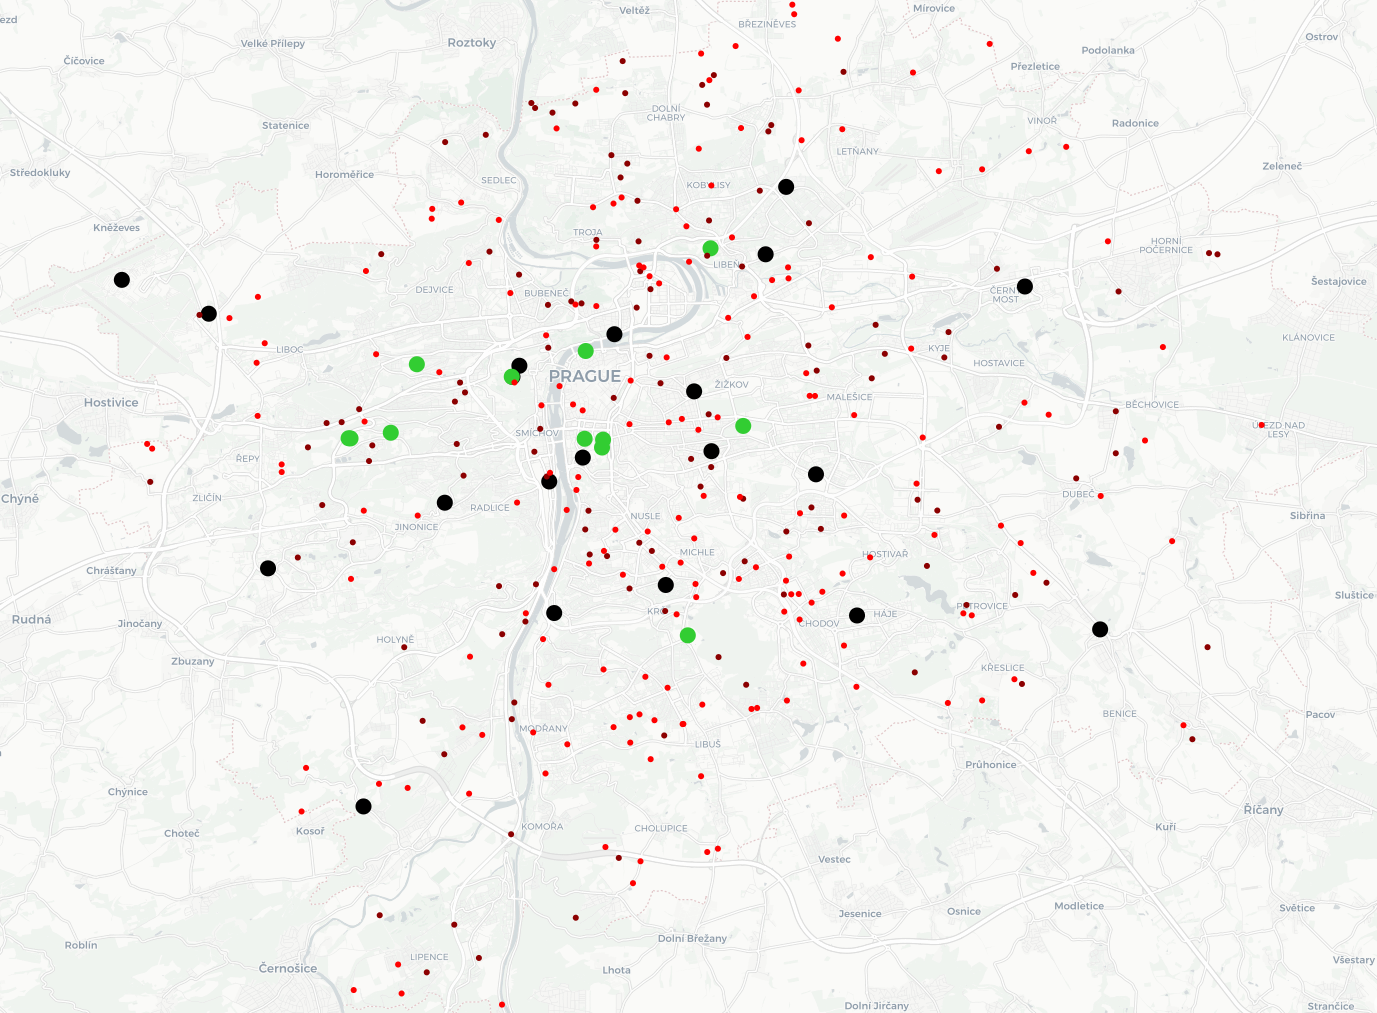
\includegraphics[width=\textwidth]{img/prague_monday_420.png}
  \centering
  \label{img:prague}
\end{figure}

Na obrázku \ref{img:prague} je znázorněno na mapě Prahy rozmístění 20 výjezdových stanic (body černé barvy), 12 nemocnic (body zelené barvy) a 300 incidentů (body červené barvy).
Tmavě červené body reprezentují incidenty, které se odehrají mezi 9 a 12 hodinou.

S výše popsanou reprezentací pohotovostní služby a sady incidentů je třeba zajistit, aby simulace uměla věrohodně zjistit doby trvání příjezdů.
Připomeňme si, že simulaci používáme právě z toho důvodu, aby počet úspěšně odbavených incidentů plánem byl co nejvěrohodnější.
Věrohodnost zajistíme použitím Google API pro zjišťování těchto dob příjezdu. Konkrétně pomocí Distance Matrix API a Routes API.

V průběhu simulace je potřeba především znát následující doby příjezdů:
\begin{enumerate}
  \item z výjezdové stanice na incident,
  \item z incidentu do nemocnice,
  \item z nemocnice zpět na výjezdovou stanici.
\end{enumerate}

Simulace podporuje i tzvn. \textit{reroute}, tedy jak se záchranný tým vrací po odbavení incidentu zpět na výjezdovou stanici,
tak je povoleno, aby mohlo z aktuální lokace vyrazit na odbavování incidentu, aniž by se musela na výjezdovou stanici vrátit.

Doby příjezdů mezi výjezdovými stanicemi, incidenty a nemocnicemi si můžeme předpočítat, ale \textit{reroute} předpočítat nelze.
Můžeme si alespoň v průběhu simulování všechny spočítané doby příjezdů mezi lokacemi udržovat s přesností na desítky metrů,
aby se v budoucnu nemuselo volat Google API, což je samozřejmě pomalá operace, trvající desítky až stovky milisekund. 

\section{Aplikace prohledávání plánů optimálními \linebreak tahy}

První metodu, kterou aplikujeme na namodelovanou záchrannou službu a incidenty podle předchozí kapitoly je algoritmus prohledávání plánů optimálními tahy \ref{alg:rekProhPlanu}.
Konkrétně použijeme jeho upravenou verzi, kde strom tahů budeme prohledávat vždy od prázdného plánu, a na každé hladině rekurze zvolíme pouze jeden náhodný optimální tah.
Oproti postupnému prohledávání všech tahů na každé úrovni má výhodu ve vyzkoušení více odlišných konfigurací a nalezené optimální plány v ceně budou s menší pravděpodobností sdílet
podobně naalokované týmy, vozidla a směny, což povede k diversifikovanějšímu prohledání množiny povolených plánů.

\begin{table}[h!]
\centering
\begin{tabular}{|c|c|c|}
\hline
\textbf{Čas běhu v minutách} & \textbf{Cena plánu} & \textbf{Odbavené incidenty} \\
\hline
7:38  & 2520055 & 295 \\
\hline
10:36 & 2325655 & 292 \\
\hline
13:23 & 2412060 & 294 \\
\hline
15:34 & 2455258 & 295 \\
\hline
17:37 & 2325654 & 288 \\
\hline
19:27 & 2505663 & 295 \\
\hline
21:20 & 2340053 & 288 \\
\hline
23:05 & 2390458 & 292 \\
\hline
24:51 & 2556061 & 295 \\
\hline
26:27 & 2325655 & 290 \\
\hline
28:10 & 2325653 & 286 \\
\hline
\end{tabular}
\caption{Spuštění prohledávání optimálními tahy na modelu Prahy.}
\label{table:optimalMovesTabulka}
\end{table}

Po spuštění metody na modelu Prahy po dobu téměř 30 minut metoda celkem navštívila 11 plánů optimálních v ceně.
Nalezený optimální plán odbavuje 295 incidentů a stojí 2455258 (viz tabulka \ref{table:optimalMovesTabulka}).
Dále má naalokovaných 101 týmů a 58 záchranných vozidel.

První plán trvá nalézt nejdelé, něco přes 7 minut. Důvodem je, že \textit{cache} dob příjezdů obsahuje pouze předpočítané hodnoty a musí se vykonávat větší množství
dotazů na Google API.
Při prohledávání dalších plánů už se dotazuje na Google API mnohem méně často.
Obodbně bude vyhodnocování prvních navštívených plánů trvat i u ostatních metod.

Metoda navštívila pro každý plán optimální v ceně při jeho budování jeden plán pro každý incident, čili celkově navštívila $11 \cdot 300 = 3300$ plánů.
Celkový počet dotazů na dobu trvání příjezdu je 133189050, kde pro 133179688 případu, tedy $99.99\%$, byla doba příjezdu předpočítaná a vrácena z \textit{cache}.

\section{Aplikace lokálního prohledávání}

V této kapitole aplikujeme na model Prahy lokální prohledávání (viz kapitola \ref{kap:localSearch}).
Použijeme ho přesně jak je popsaný algoritmem \ref{alg:hillclimb}.
Prohledávání začneme z prázdného plánu a jako účelovou funkci použijeme váženou sumu ceny plánu a počtu odbavených incidentů, s parametrem $\alpha = 0.99$ (viz definice \ref{df:vazenaSumaUcelF}),
abychom upřednostňovali plány s vyšším počtem odbavených incidentů.
Jakou přesně účelovou funkci si zvolíme uvážíme podle toho, co pro nás konkrétně znamená optimální plán. My budeme chtít zkoumat především plány odbavující co nejvíce incidentů a až poté minimalizovat cenu.

Potřebujeme ještě nadefinovat jak budou vypadat sousedi nějakého plánu.
Ty standardně nadefinujeme implicitně pomocí tahů a vyžadujeme, aby splňovali alespoň nutné podmínky.
Takové tahy můžeme vybrat různě, my si vybereme tahy uvedené jako příklad tahů, které splňují nutné podmínky (viz příklad \ref{pr:sousedi}).

Záměrně alokování týmu a vozidla zvolíme jako jeden tah a nikoliv jako dva samostatné tahy. Vyhneme se tak situaci, kdy by se lokální prohledávání zastavilo v lokálním optimu, 
kde už nelze odbavit žádný incident naalokování týmu a vozidla odděleně, ale pouze zároveň. Takové lokální optimum by pak bylo suboptimální, protože by odbavovalo méně incidentů, než by mohlo být možné.
Takto definované sousedství budeme používat i u dalších metod.

\begin{figure}[H]
  \caption{Nalezené plány metodou lokálního prohledávání plánů.}
  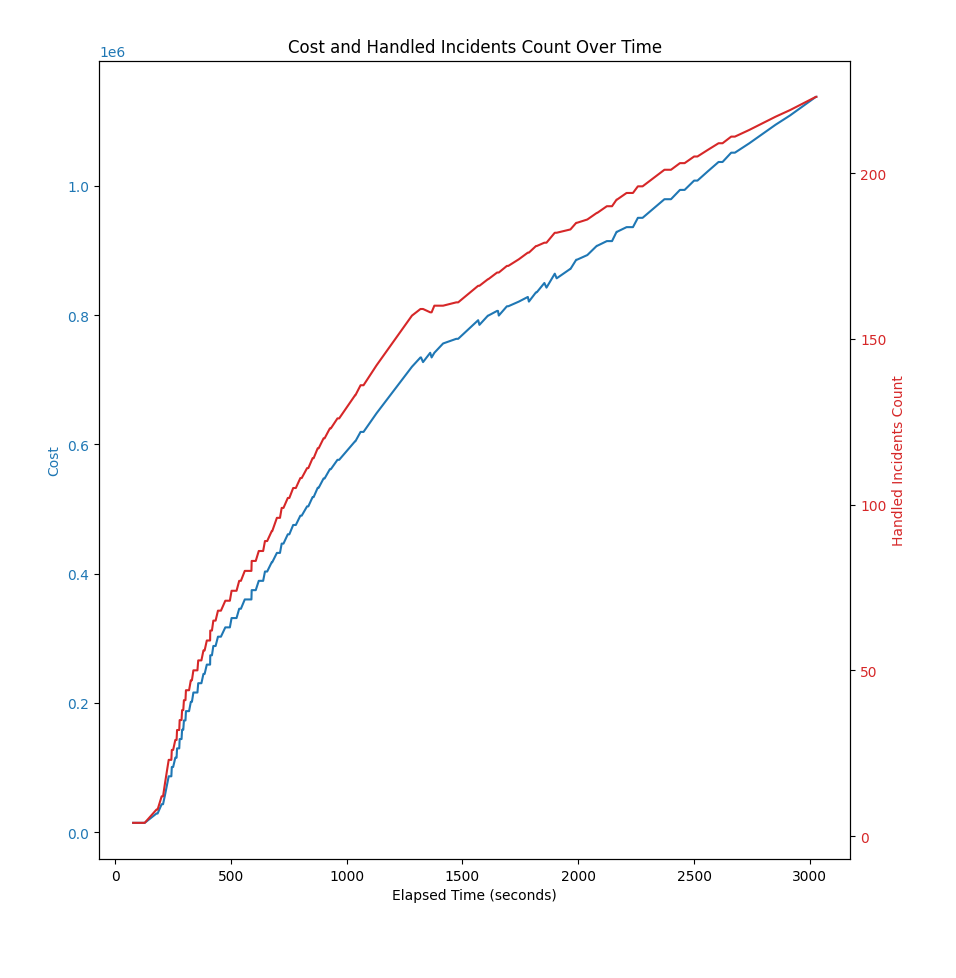
\includegraphics[width=\textwidth]{img/local_search_empty_plan_plot.png}
  \centering
  \label{img:localSearchRes}
\end{figure}

Na obrázku \ref{img:localSearchRes} vidíme jak se aktuální plán mění v čase.
Lokální prohledávání bylo spuštěné po dobu 50 minut, a pak bylo přeřušeno. 
Nejlepší nalezený plán po 50 minutách úspěšně odbaví 223 incidentů z 300 incidentů a stojí 137673.
To je v porovnání s předchozí metodou, která za pouhých 7 minut nalezla plán odbavující 295 incidentů nedostačující výsledek.
I když by se podle růstu křivky dalo usoudit, že by metoda lokálního prohledávání také byla schopná nalézt dost dobrý plán, trvalo by to příliš dlouho.

Lokální prohledávání celkem navštívilo 22997 plánů. To je až 7 krát tolik, kolik plánů navštívila metoda prohledávání optimálními tahy.
Lokální prohledávání tedy není vhodné na budování optimálního plánu z prázdného plánu, protože zbytečně navštíví velké množství plánů a trvá tak zbytečně dlouho.

Můžeme si polepšit, sice že začneme prohledávát ne z prázdného plánu, ale z plánu zvoleného nějak chytře. Z plánu, který už je skoro optimální a lokální Prohledávání
už jej jenom doladí.

Jednou z možností jak takový startovní plán zvolit je použít první nalezený optimální plán v ceně předchozí metodou a na něj spustit lokální prohledávání.

\begin{figure}[H]
  \caption{Nalezené plány metodou lokálního prohledávání plánů z plánu optimálního v ceně.}
  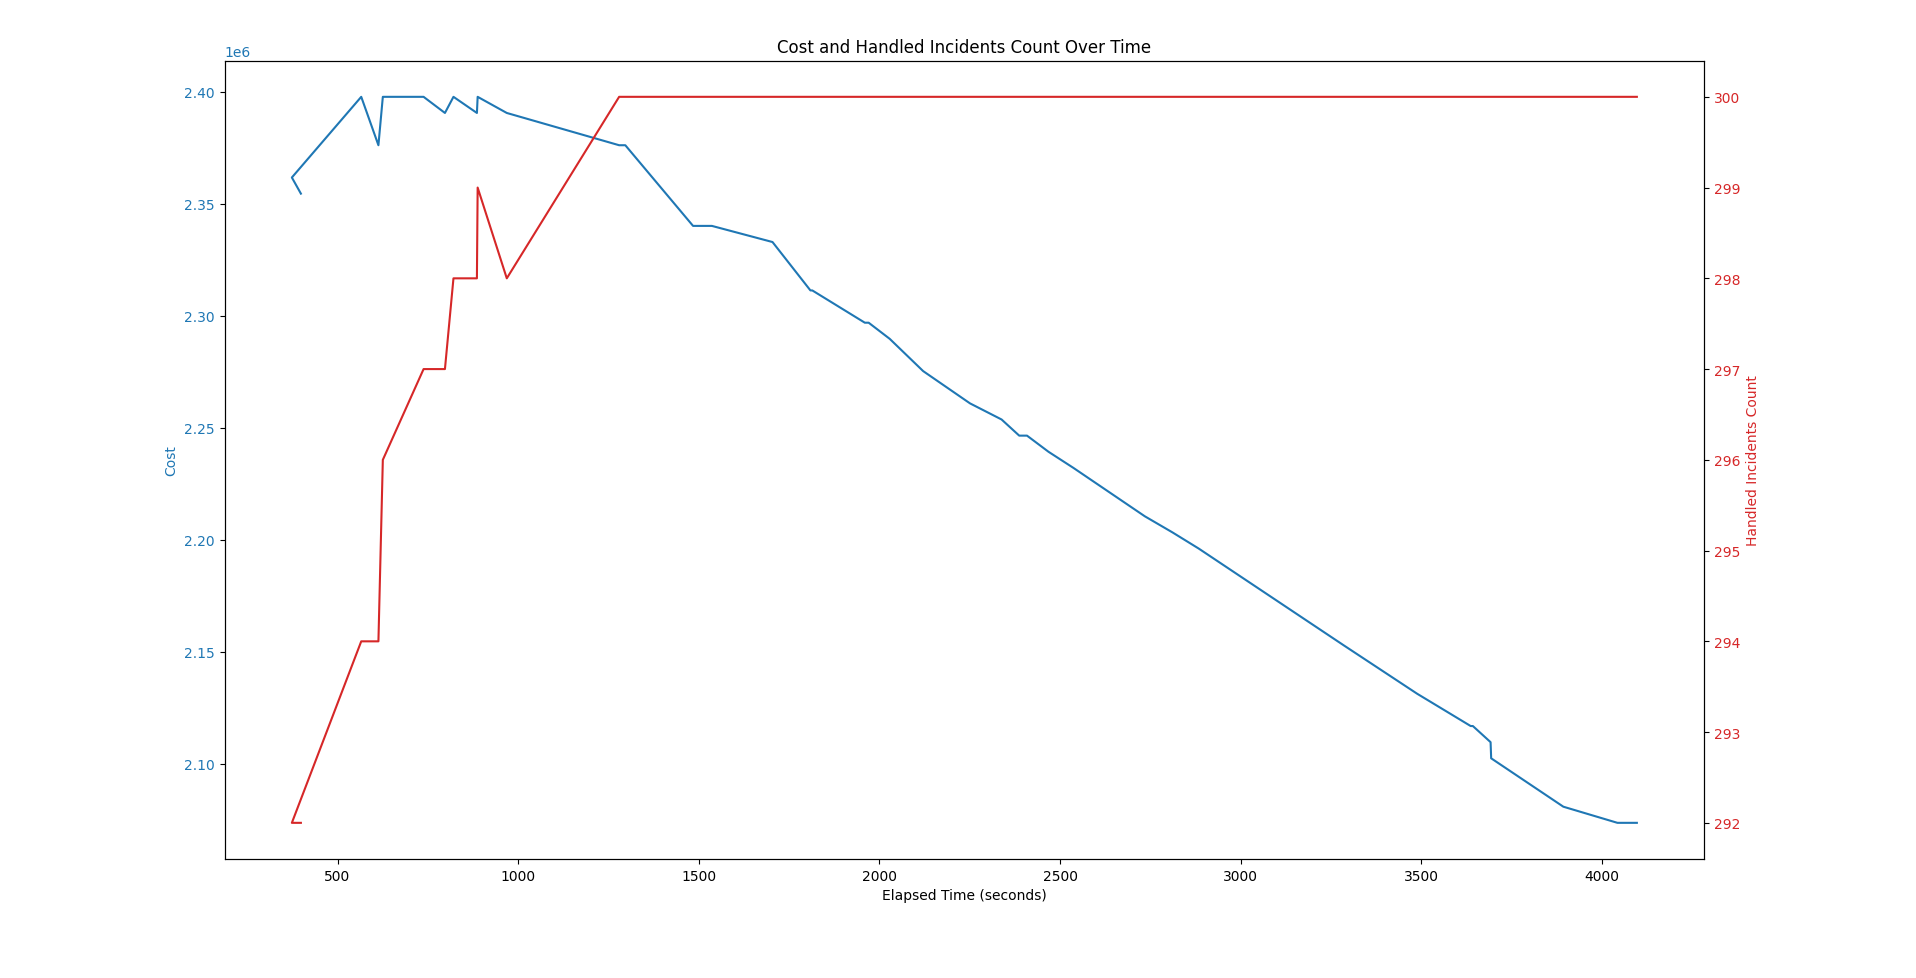
\includegraphics[width=\textwidth]{img/hybrid_prague.png}
  \centering
  \label{img:hybrid}
\end{figure}

Na obrázku \ref{img:hybrid} vidíme graf, kde lokální prohledávání začíná ne z prázdného plánu, ale z plánu optimálního v ceně.
Můžeme vidět, že lokální prohledávání upravuje plán tak, že postupně odbavuje více incidentů, až nakonec všech 300. Poté už jen postupně snižuje cenu plánu.
Po 20 minutách nalezne plán odbavující všechny incidenty a zhruba po hodině lokální prohledávání stagnuje a nalezne lokální optimum.
Optimální nalezený plán odbavuje všech 300 incidentů, stojí 2073655 a má naalokovaných pouze 87 týmů a 55 vozidel.

\section{Aplikace tabu prohledávání}

V této kapitole aplikujeme na model Prahy tabu prohledávání (viz kapitola \ref{kap:tabuSearch}).
Tabu prohledávání je v podstatě lokální prohledávání s pamětí, podle které umí sofistikovaněji vybrat sousední plán,
pokud se ocitne v lokálním optimu.
Z toho důvodu bude podobně jako u lokálního prohledávání trvat příliš dlouho, než nalezne nějaký dost dobrý plán, pokud bychom tabu prohledávání pustili z prázdného plánu.
Nemá proto smysl pouštět tabu prohledávání z prázdného plánu a pustíme tabu prohledávání rovnou z nějakého už dost dobrého plánu.
Tím bude stejně jako u lokálního prohledávání plán optimální v ceně.

\begin{figure}[H]
  \caption{Nalezené plány tabu metodou z plánu optimálního v ceně.}
  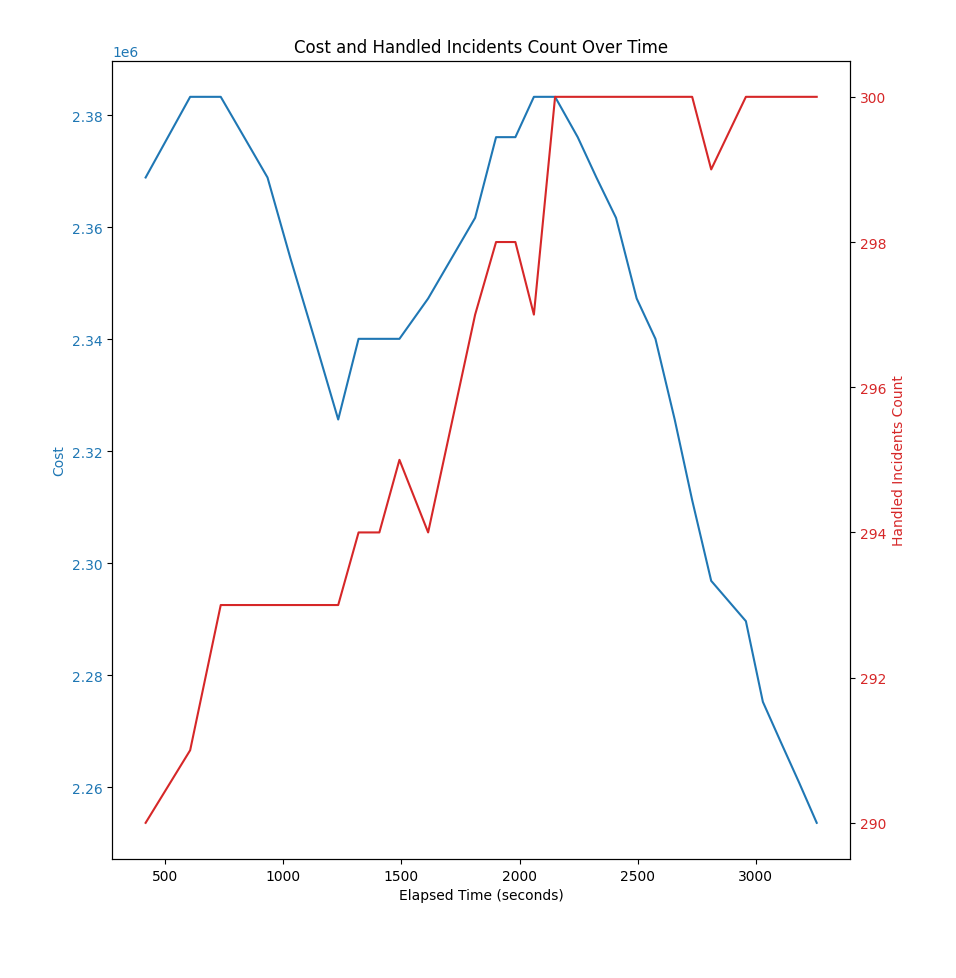
\includegraphics[width=\textwidth]{img/prague_hybrid_tabu.png}
  \centering
  \label{img:hybrid_tabu}
\end{figure}

Na obrázku \ref{img:hybrid_tabu} vidíme doposud nejlepší plány nalezené tabu metodou v čase.
Nalézt plán odbavující všech 300 incidentů trvá kolem 30 minut, což je o 10 minut déle, než trvalo lokálnímu prohledávání. 
To je pochopitelné, protože při navštívení každého souseda, kterých bude obdobně jako u lokálního prohledávání, se musí kontrolovat,
zda není obsažen v tabu. Proto vyhodnocení souseda bude trvat o něco déle, což se při tak velkém množství navštívených plánů poměrně rychle nasčítá.

Tabu prohledávání bylo puštěno něco kolem hodiny, a obdobně jako u lokálního prohledávání, s roustoucí délkou běhu programu se i snižuje cena plánu.
Výhoda tabu prohledávání je hlavně v schopnosti nezůstat v lokálním optimu a umět robustněji prohledávat prostor konfigurací.
Tato výhoda v našem případě ale není využita, protože tabu prohledávání ani za hodinu běhu na lokální optimum nenarazilo.
Spíše naopak, prohledávání tabu je nevýhodou, a lokální prohledávání je v tomto případě lepší volbou.

\section{Aplikace simulovaného žíhání}

V této kapitole aplikujeme na model Prahy simulované žíhání (viz kapitola \ref{kap:tabuSearch}).
Simulovanému žíhání je potřeba nastavit následující hyperparametry:
\begin{enumerate}
  \item počáteční teplota,
  \item koncová teplota,
  \item chladící rozvrh.
\end{enumerate}

Počáteční teplota je vhodné nastavit tak, aby pravděpodobnost přijetí horší konfigurace byla ze začátku kolem 0.8--0.9 procent \cite{sa_theory}.
Vzhledem k tomu, že používáme váženou sumu účelových funkcí, tak se výsledná hodnota účelové funkce pohybuje mezi 0 a 1.
Tím pádem rozdíl se pohybuje mezi -1 a 1.
Pokud je $\Delta$ záporná, tak je sousední plán vždy navštíven, protože je
jeho hodnota při účelové funkci vyšší. Zajímá nás tedy pouze případ, kdy je $\Delta$ nekladná.

Připomeňme si jak vypadá akceptační kritérium:
\begin{align*}\label{df:metropolis}
  \exp\left(-\frac{\Delta q}{t}\right).
\end{align*}

Počáteční teplota splňující takový požadavek činí například 5 stupňů, jak můžeme vidět na obrázku \ref{img:metropolis_5},
kde na ose x je hodnota delta, a na ose y pravděpodobnost přijetí sousedního plánu metropolisním kritériem, který se od aktuálního liší o danou deltu.

\begin{figure}[H]
  \caption{Metropolis kritérium pro teplotu 5 stupňů.}
  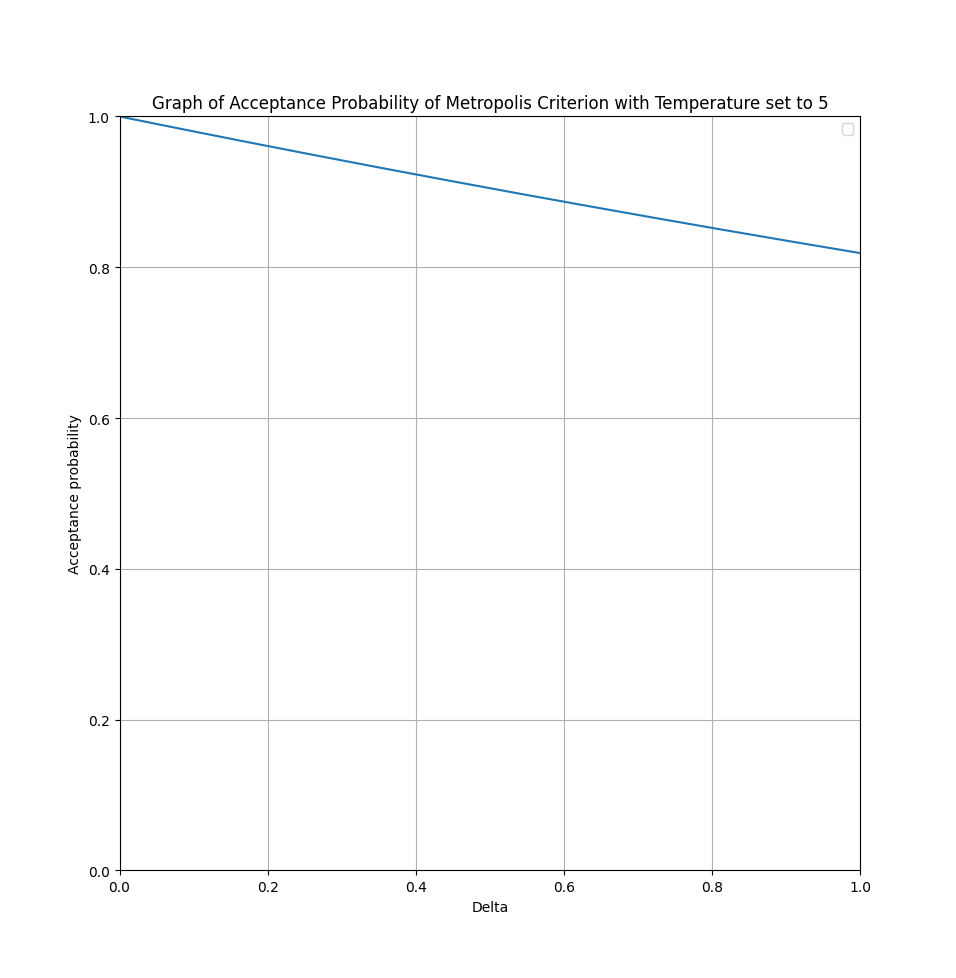
\includegraphics[width=\textwidth]{img/metropolis_5.png}
  \centering
  \label{img:metropolis_5}
\end{figure}

Finální teplota se často volí velmi blízko nule, aby bylo možné dostatečně důkladně prohledat konfigurace lokálně, podobně jak dělá například lokální prohledávání \cite{sa_theory}.
Vyberme finální teplotu jako $10^{-6}$.

Vybrat ochlazovací rozvrh lze různě, nejčastěji používané jsou \cite{sa_theory}:
\begin{enumerate}
  \item Lineární chladící rozvrh, kde se teplota aktualizuje následovně:
    \begin{align*}
      t_{k+1} = t_k - k \cdot \Delta t_k,
    \end{align*}
    kde $t_k$ je aktuální teplota, $t_{k+1}$ je nová teplota a $\Delta t_k$ je hyperpametr, o kolik teplotu snižovat.
    Je velmi jednoduchý na implementaci, ale není tak dobrý jako ostatní ochlazující rozvrhy \cite{sa_schedules}.

  \item Logaritmický ochlazující rozvrh:
    \begin{align*}
      t_{k+1} = t_{k} / \log(1 + k).
    \end{align*}
    Logaritmický ochlazující rozvrh má dobré teoretické vlastnosti, ovšem pro praktické použití je příliš pomalý \cite{sa_schedules}.

  \item Exponenciální ochlazující rozvrh:
    \begin{align*}
      t_{k+1} = t_k \cdot \alpha,
    \end{align*}
    kde $\alpha$ se často volí mezi 0.8 a 0.99 \cite{sa_theory}.
    Podobně jako předchozí ochlazující rozvrhy je velmi jednoduchý na implementaci, a často bývá dobrou první volbou, protože umí najít dobrý balanc mezi explorační fází,
    kdy je teplota vyšší a mezi ladící fází, kdy je teplota nižší \cite{sa_theory}.

  \item Adaptující se ochlazující rozvrh. Algoritmus si sám v průběhu nastavuje teplotu podle chování a doposud nalezených konfigurací.
    Náročnější na implementaci než předchozí ochlazující rozvrhy. Hodí se uvažovat o jeho použití především, pokud jednodušší ochlazující rozvrhy nalézají pouze suboptimální řešení.
\end{enumerate}

My si jako ochlazovací rozvrh zvolíme exponenciální ochlazovací rozvrh, především pro jeho jedhoduchou implementaci a pěkné vlastnosti.
Jako první spustíme simulované žíhání z prázdného plánu.

\begin{figure}[H]
  \caption{Simulované žíhání z prázdného plánu.}
  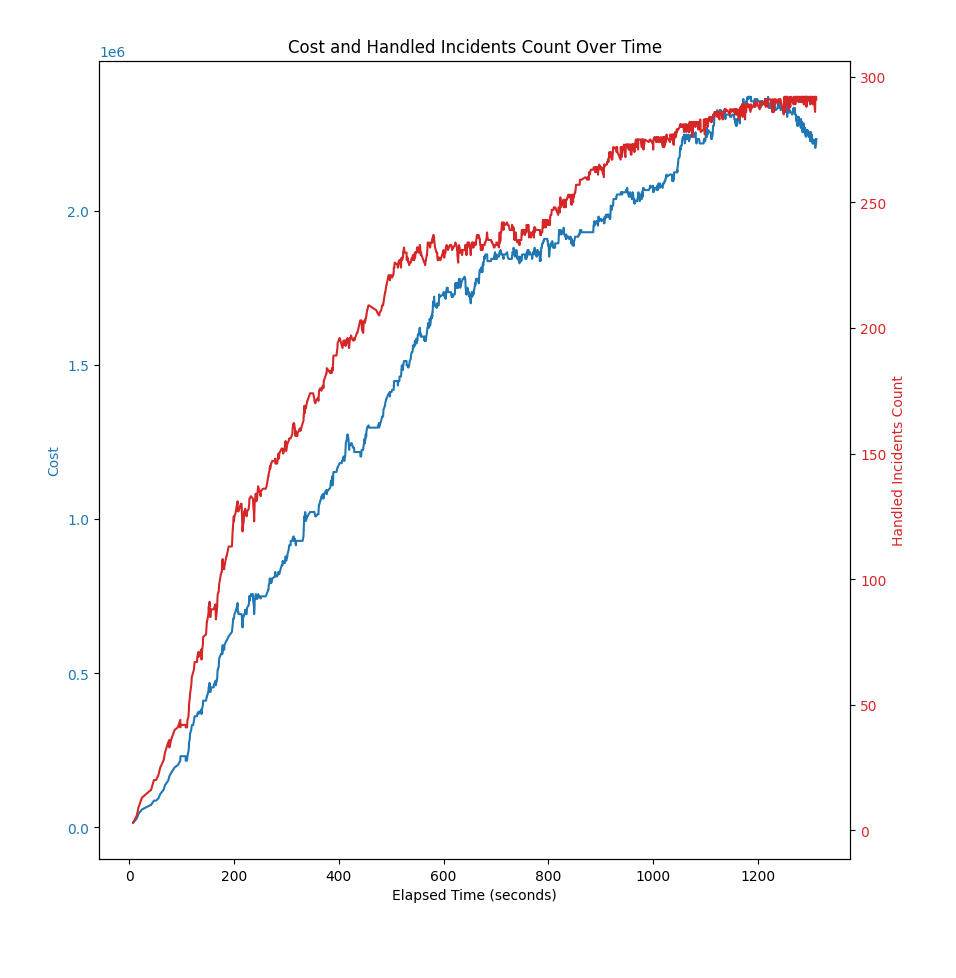
\includegraphics[width=\textwidth]{img/sa_empty_elapsed.png}
  \centering
  \label{img:sa_empty}
\end{figure}

Na obrázku \ref{img:sa_empty} vidíme, jaké plány simulované žíhání v průběhu z prázdného plánu navštěvovalo.
Celkově běželo simulované žíhání 20 minut a navštívilo celkem 1779 plánů.
Nejlepší nalezený plán odbavuje 292 incidentů, stojí 2217732 a má naalokovaných 89 týmů a 132 záchranných vozidel.
V porovnání s lokálním nebo tabu prohledáváním z prázdného plánu se jedná o dramaticky lepší výsledek.

Podobně jako u předchozích metod můžeme zkusit spustit simulované žíhání z jiného než prázdného plánu.
Zkusme spustit z uniformě náhodně vygenerovaného plánu, který má naalokovaných zhruba 50\% týmů a vozidel.

\begin{figure}[H]
  \caption{Simulované žíhání z náhodného plánu.}
  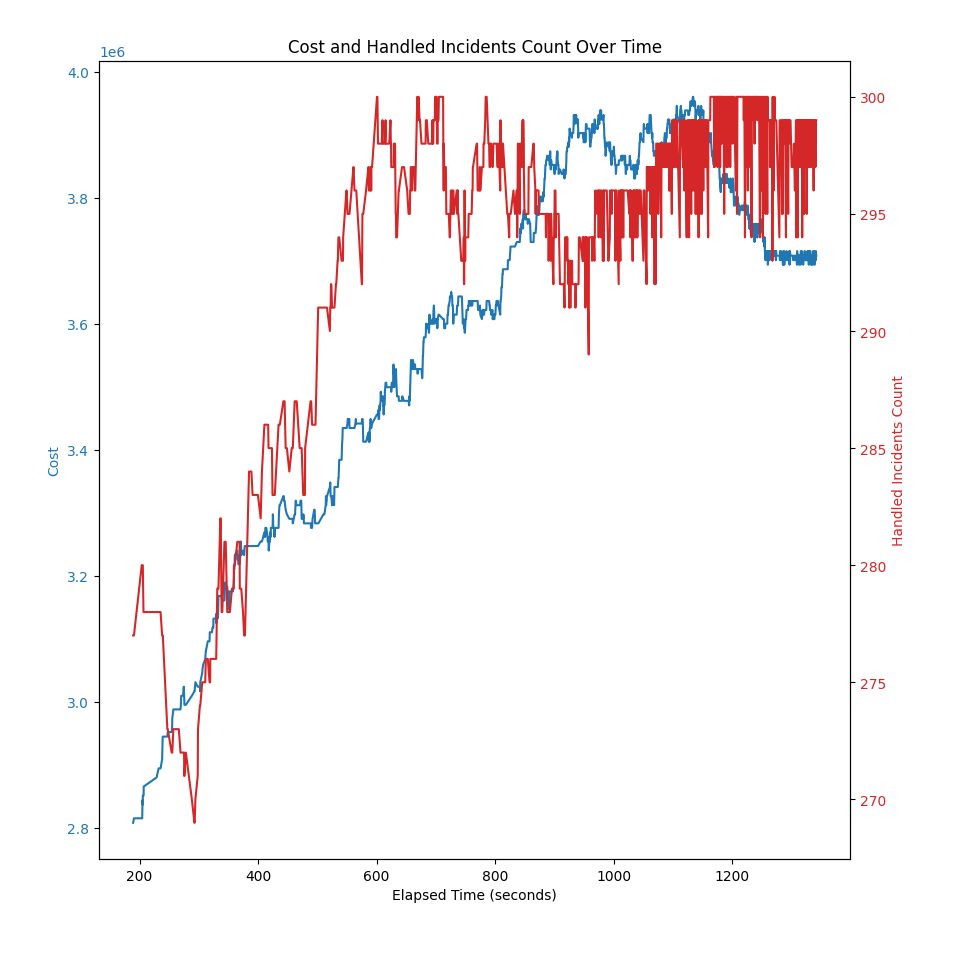
\includegraphics[width=\textwidth]{img/sa_random_elapsed.png}
  \centering
  \label{img:sa_random}
\end{figure}

Na obrázku \ref{img:sa_random} vidíme chování simulovaného žíhání spuštěného z náhodně vygenerovaného plánu.
Přibližně do 15 minuty (1000 sekund) lze vidět explorační fázi, kdy následně už je plán pouze lokálně vylepšován. 
Spustit simulované žíhání z náhodného plánu přináší lepší výsledky než z plánu prázdného.
Nejlepší nalezený plán odbavuje všech 300 incidentů, stojí 3456121 a má naalokovaných 139 týmů a 121 vozidel.

Zkusme ještě spustit simulované žíhání z plánu optimálního v ceně, podobně jako u lokálního a tabu prohledávání.

\begin{figure}[H]
  \caption{Simulované žíhání z plánu optimálního v ceně.}
  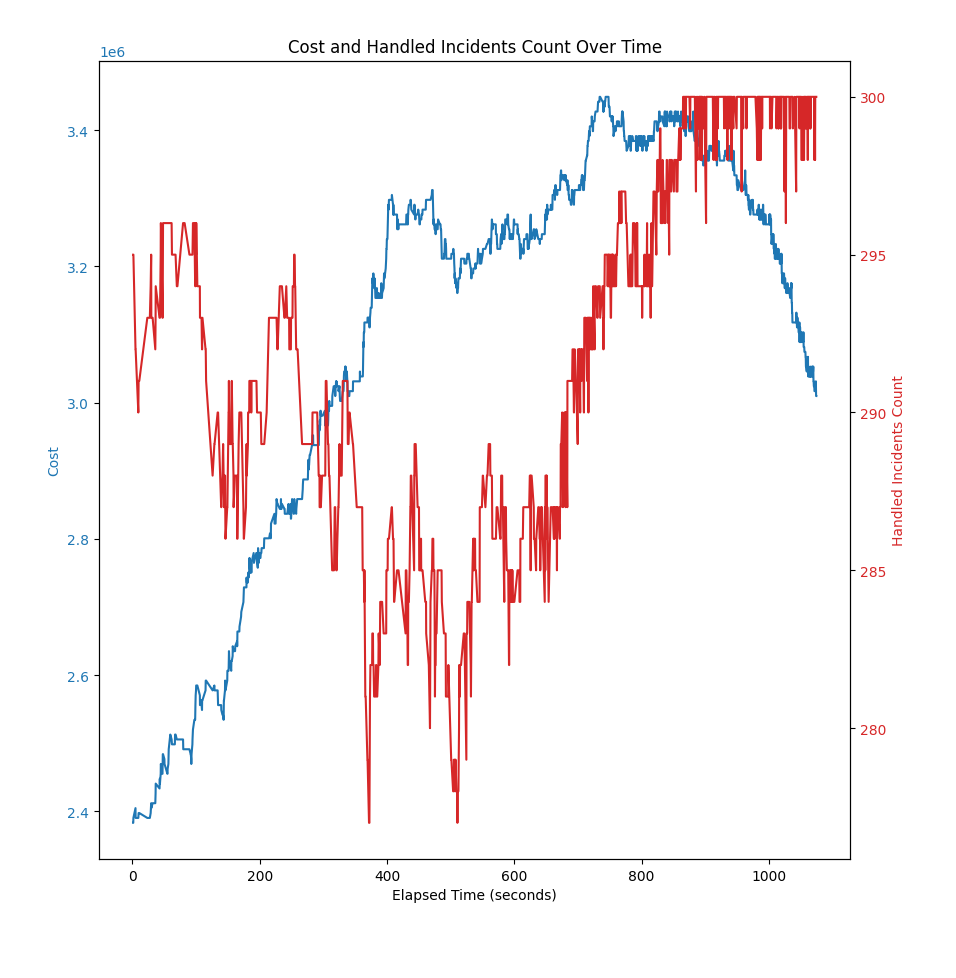
\includegraphics[width=\textwidth]{img/sa_optimal.png}
  \centering
  \label{img:sa_optimal}
\end{figure}

Na obrázku \ref{img:sa_optimal} vidíme průběh výpočtu.
Podobně jako v případě procházení z náhodného plánu jsou při vyšší teplotě navštěvovány horší plány v rámci explorace a od přibližně 
10 minuty (700 sekund) se postupně přechází do ladící fáze, která se chová podobně jako lokální prohledávání.
Program celkově běžel něco pod 30 minut i spolu s nalezením plánu optimálního v ceně.
Nejlepší nalezený plán odbavuje 300 incidentů, stojí 3009734 a má naalokovaných 110 týmu a 134 vozidel.

